% !TEX root = ../../main.tex
% !TEX spellcheck = en_US
\section{Defense manager}
\label{sec:defense_manager}
The defense manager handles the defense of its own base and the player’s base. It calculates defense
locations from BATS's and the teammate's outer choke points (marked \usebox{\LegendDotRed} and
\usebox{\LegendDotOrange} in figure \ref{fig:defense_locations}. On the red dots it places
\nameref{sec:hold_squad}s to guard the entrance and the \nameref{sec:patrol_squad} patrols between
these red dots. It does not defend a region that only abuts to BATS or teammate
occupied regions, seen as yellow outline in the figure.

The Hold squads, described fully in section \ref{sec:hold_squad}, are stationary and defend the
choke point from a certain roaming perimeter (purple circle in the figure) where the center is
calculated by finding a position in the range \squadDefendRoamDistanceMinMax~closest to one of
BATS’s or the teammate’s buildings and the radius being \squadDefendRoamPerimeter. Units from the
Hold squad will stay in the roaming perimeter until enemy units enter the defense perimeter
(\squadDefendDefendPerimeter~in radius), they will then start to attack the enemy. 

\begin{figure}[htb]
\centering
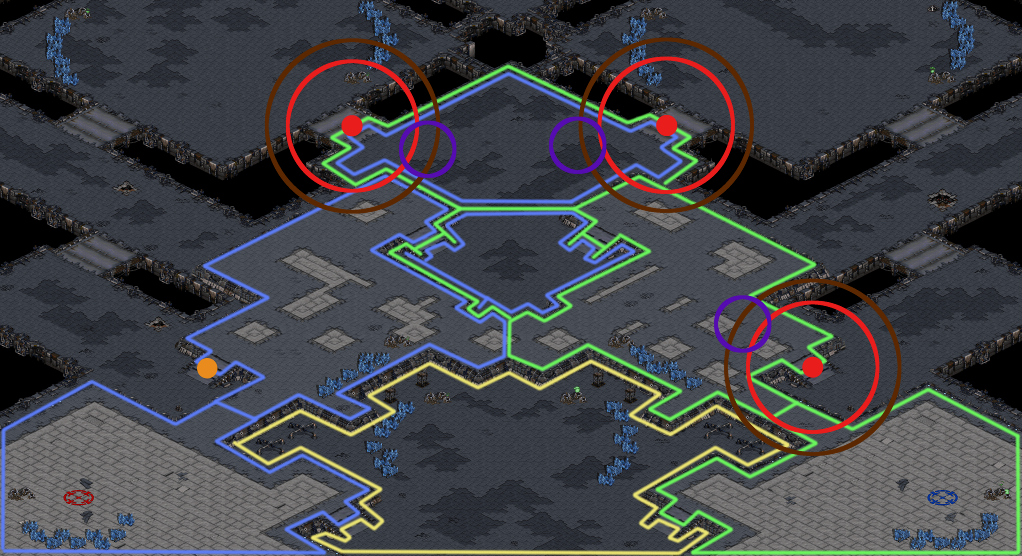
\includegraphics[width=\textwidth]{space_atoll_(co-op)_defense_locations}
\caption[Defense locations example]{
	Example of defense locations.
	\usebox{\LegendLineLightGreen} BATS’s regions;
	\usebox{\LegendLineLightBlue} teammate’s regions;
	\usebox{\LegendLineLightGreenLightBlue} belongs to both;
	\usebox{\LegendLineYellow} non-defended as they abut only BATS or teammate regions;
	\usebox{\LegendDotRed} defense locations;
	\usebox{\LegendCircleRed} defend perimeter;
	\usebox{\LegendCircleBrown} enemy offensive perimeter;
	\usebox{\LegendCircleViolet} roam location for Hold squads; and
	\usebox{\LegendDotOrange} teammate's defense location.}
\label{fig:defense_locations}
\end{figure}

Patrol squads on the other hand contains all free units and patrol between the defense locations. If
enemy units enter the enemy offensive perimeter (\squadDefendEnemyOffensivePerimeter~in radius) in a
defense location all squad units will move to the defend location to defend it, all other hold
squads will disband to join the defense with the Patrol squad. The idea was first to only disband
the other Hold squads if the enemy is too strong, but the calculation proved to be more time
consuming than guessed, thus we focused work on other more important areas. The strategy was tested
and works good against one StarCraft default bot, as it only attacks from one location at a time.
Two default bots can however attack from different locations, but usually attacked from one
location. Two bots were, however, often too strong for BATS to defend by itself. Although the
strategy worked against the default bot it would probably not work against other bots or humans that
can attack two different locations simultaneously.

Both Hold squads and Patrol squads roam or patrol between BATS’s defense location, meaning the bot
will not disturb the teammate with its units.

\paragraph{Defending other locations}
Although no Hold squads are located on and the Patrol squad never patrols between the teammates
defend locations. It will still send the Patrol squad to defend a teammate defend locations if BATS
is not under attack itself. In addition to defending all defend locations, the defense manager will
send out the Patrol squad to defend locations either inside BATS’s or the teammate's base that are
under attack, for example if the enemy drops inside the base. This will, however, never bring the
Hold squads as they should defend the entrance to the base.
